\chapter{Desenvolvimento}
\label{desenvolvimento}

Este capítulo refere-se a execução da proposta apresentada no capitulo \ref{proposta}, correspondendo ao fluxo de desenvolvimento indicado na seção \ref{fluxo_desenvol} deste trabalho. Será abordado como foi o processo de desenvolvimento do sistema de recomendação proposto, assim como as dificuldades e alterações realizadas sobre a proposta inicial para sua maior integridade.

Seguindo a metodologia \textit{Scrum}, foi realizado o \textit{backlog} do produto inicial (encontrado no apêndice \ref{apendice_backlog_inicial}), contendo as \textit{stories} descritas em \ref{section_product_backlog}, juntamente com as \textit{sprints} e as prioridades de cada \textit{story}.

O capítulo foi dividido por \textit{sprints} presentes no \textit{backlog} do produto, sendo apresentado ao final os artefatos gerados e uma breve discussão. No desfecho do capítulo será exibido as análises gerais realizadas no trabalho.

\section{1º \textit{Sprint}}

Na primeira \textit{sprint}, foram criados novos componentes no \textit{front-end} da Liva e feitas alterações nas páginas, inclusive correções de \textit{bugs} para se adequarem ao novo sistema de recomendação que irá entrar em produção após sua conclusão. Essas alterações são tais como: design da modal de alteração do perfil de busca (Figura \ref{fig:componente_busca}) e a adição do novo componente de apresentação de imoveis recomendados, além do sistema de comunicação implementado para transmissão de dados de ações dos clientes para API.

\begin{figure}[H]
    \centering
    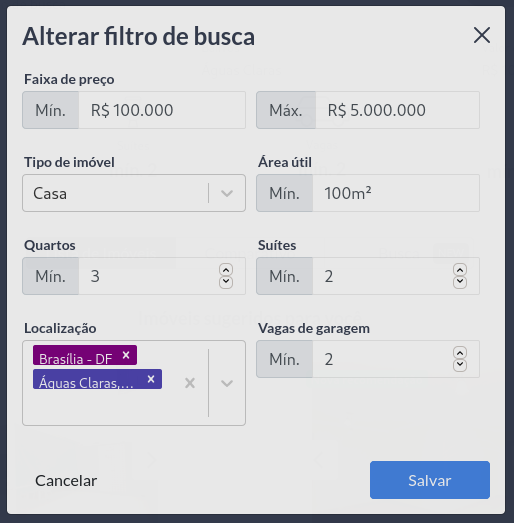
\includegraphics[scale=0.45]{figuras/desenvolvimento/componente_busca.png}
    \caption[Modal de alterar filtro de busca]{Modal de alterar filtro de busca.}
    \label{fig:componente_busca}
\end{figure}

Também foi realizada a configuração da integração e \textit{deploy} contínuo utilizando a ferramenta Actions do próprio Github, sendo nele realizado a execução dos testes unitários e a execução do \textit{deploy} automático no AWS.

O componente de apresentação de imóveis que anteriormente tinha sido colocado na lateral da página de detalhes, atualmente foi inserido de forma a ocupar a largura toda do corpo da página como pode ser visto na Figura \ref{fig:componente_ml}, pois dessa forma o usuário consegue ver várias recomendações ao mesmo tempo, sem precisar ficar clicando mais vezes para ver recomendações. Antes, ele tinha sido colocado na lateral da página de detalhes, ao lado do mapa de localização, por razão de menor ocupação do espaço da página, como foi apresentado na Figura \ref{fig:prototipo_recommender_system}.

No componente são apresentados 5 novas propriedades para o usuário, no qual é possível rolar os \textit{cards} de imóveis com as setas horizontais. Em cada \textit{card} é exibido as seguintes características: imagens da propriedade, preço, tipo de imóvel, cidade em que o imóvel é localizado, quantidade de quartos, quantidade de suítes, quantidade de área e quantidade de vagas de garagem.

\begin{figure}[H]
    \centering
    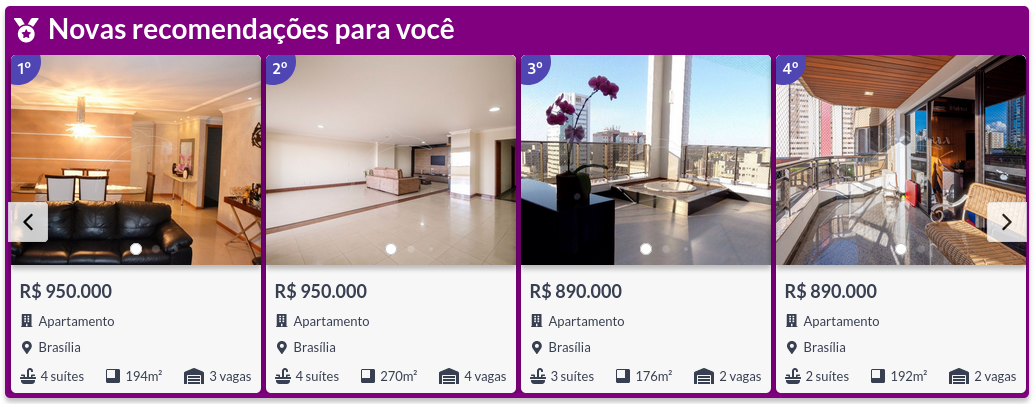
\includegraphics[scale=0.42]{figuras/desenvolvimento/componente_ml.png}
    \caption[Componente de apresentação de imóveis recomendados]{Componente de apresentação de imóveis recomendados.}
    \label{fig:componente_ml}
\end{figure}

Na implementação do registro das ações dos usuários foi notado que não era necessário o uso da ferramenta KINESIS do AWS, pois foi percebido que para transmissão de dados desse tipo não havia a necessidade de uma ferramenta tão poderosa. Essa ferramenta do AWS normalmente é utilizada para transmissão de vídeos e outros dados mais pesados, conseguindo capturar continuamente gigabytes de dados por segundo de centenas de milhares de origens \cite{KINESIS:2019}.

Ao final da \textit{sprint}, na reunião de \textit{sprint review} foi decidido que era necessário criar uma nova \textit{story} para substituir a tecnologia KINESIS da AWS.

\subsection{\textit{Sprint backlog} e resultados}

O quadro \ref{quadro:sprint1} referente a primeira \textit{sprint}, demonstra as \textit{stories} concluídas, pendentes e as novas que surgiram na reunião de \textit{sprint planning}. Para essa \textit{sprint} surgiram as \textit{stories} técnicas TS08 e TS06 pela necessidade da melhora do design dos componentes de perfil de busca e crítica. Também surgiram as \textit{stories} TS12 E TS13, referentes a construção de um CI/CD, que são muito importantes para a manutenção contínua do software.

\begin{quadro}[H]
\centering
\caption[\textit{Sprint backlog} e resultados da \textit{sprint} 1]{\textit{Sprint backlog} e resultados da \textit{sprint} 1.}
\label{quadro:sprint1}
\begin{tabular}{|p{6cm}|p{2cm}|p{2cm}|p{1cm}|}
\hline
\multicolumn{1}{|c|}{\textbf{Stories planejadas}} & \multicolumn{1}{c|}{\textbf{Concluídas}} & \multicolumn{1}{c|}{\textbf{Pendentes}} & \multicolumn{1}{c|}{\textbf{Novas}} \\ \hline
US01 - Visualizar perfil de busca & X &  &  \\ \hline
US02 - Alterar perfil de busca & X &  &  \\ \hline
TS01 - Corrigir bugs existentes na página de detalhes do imóvel & X &  &  \\ \hline
TS02 - Corrigir bug de agendamento de visitas & X &  &  \\ \hline
TS03 - Registrar ações do usuário no sítio virtual &  & X &  \\ \hline
TS08 - Melhorar design do componente de recomendação & X &  & X \\ \hline
TS06 - Melhorar design da modal do perfil de busca & X &  & X \\ \hline
TS07 - Melhorar design do componente de crítica & X &  & X \\ \hline
TS12 - Configurar integração contínua & X &  & X \\ \hline
TS13 - Configurar deploy automático & X &  & X \\ \hline
\end{tabular}
\end{quadro}

\section{2º \textit{Sprint}}
\label{sprint2}

Para a segunda \textit{sprint} como descrito anteriormente, a \textit{story} de registro de ações dos usuários permaneceu pelo fato de haver a necessidade da troca de tecnologia para as transmissões de dados. Foi realizado também, o início da coleta de dados para o módulo de aprendizado de máquina.

Os \textit{sockets} TCP são mensageiros instantâneos que conseguem trazer de maneira rápida e garantida a entrega de dados. Uma forma de visualizar o funcionamento de socket TCP seria compará-lo a uma ligação telefônica onde alguém faz uma ligação para outra pessoa e quando esta atende, é criado um canal de comunicação entre os dois falantes. \cite{Carla:2005}

Dessa forma, a transmissão de dados seria mais adequada com o uso do protocolo via \textit{web socket}. Com isso, foi utilizada a biblioteca \textit{channels} para criar os "consumidores" na API e a biblioteca "socket.io" para utilização do \textit{socket} no \textit{front-end}. Assim, os dados são enviados em tempo real sem custo adicional de outra ferramenta e atendendo a demanda existente.

Desde o início do desenvolvimento existia a necessidade de coletar uma base de dados inicial para treinar o modelo e assim tê-lo eficiente com boas recomendações assim que entrasse em produção. Com isso, a ideia inicial era a de implementar uma captura de dados de conversões (CVs), \textit{likes}, \textit{dislikes} e perfis de busca no site da Liva e deixar o tempo o suficiente para obtenção de uma base de dados robusta. Mas devido a alguns fatores, o fluxo de pessoas no site da Liva diminuiu drasticamente, impossibilitando pôr em prática essa estratégia descrita anteriormente para obtenção dessa base de dados robusta inicial.

Dessa forma, houve a necessidade de uma nova estratégia para obtenção da base inicial. Após algum tempo analisando possibilidades foi escolhido um novo plano, que consistiu na utilização da base de dados dos \textit{Leads}, adaptado para o modelo proposto.

Como os \textit{Leads} são conversões (CVs) advindos de outras plataformas eles continuam sendo uma fonte valiosa de dados para o modelo proposto. Dessa forma, o novo plano baseia-se em manipular essa base de dados para se adequar ao modelo. Com a existência de dois tipos de \textit{Leads}, primeiro e segundo contato, há a possibilidade de criar o que seriam os cliques em propriedades do cliente com os \textit{Leads} de segundo contato. O \textit{Lead} de primeiro contato seria o primeiro de um cliente demonstrando interesse em uma propriedade, enquanto o \textit{Lead} de segundo contato são referentes aos \textit{Leads} de clientes já cadastrados, ou seja, a partir da sua segunda interação. O "candidato" ou propriedade convertida seria a última propriedade de segundo contato. Com a  existência do perfil de busca em cada \textit{Lead} não houve problema com as \textit{features} iniciais relacionadas ao perfil de busca.

Assim, foi feito um \textit{script} na linguagem Ruby que foi executado no ambiente de produção da Liva, manipulando a base de dados dos \textit{Leads}, incluindo uma "limpeza" nos dados, retirando dados de teste, repopulando campos nulos a partir de contato direto com as imobiliárias, adaptando os dados de classes e adicionando os perfis de busca. Com isso foi criada uma nova base de dados de conversões positivas, ou seja, com alvo igual a 1 ou CV igual a 1. Como todo modelo que irá classificar a probabilidade de um evento, há a necessidade de dados que representam a "não conversão" de propriedades, e isso a base de dados dos\textit{Leads} não consegue proporcionar.

Por isso uma estratégia foi escolhida para popular a nova base de dados com "não conversões", ou de alvo 0. Ela consiste em, como igualmente uma estratégia adotada pelo \textit{site} Summo.jp, a cada uma conversão de alvo 1, dez não conversões ou de alvo 0 são criadas, como descrito em (\ref{design_modelo}). Dessa forma foi possível a geração de uma base de dados inicial com 80300 tuplas aproximadamente.

Com a base de dados inicial obtida foi possível notar um desbalanceamento dos dados, pois existem mais alvos 0 do que 1. Neste caso, o desbalanceamento vem como algo positivo, pois na natureza do problema, em que existe uma conversão de um imóvel e outras 10 "não conversões" de outros imóveis para as mesmas \textit{features} relacionadas as pesquisas e interesses do usuário a ideia pode ser generalizada para o caso em que cada usuário tende a apresentar muitos comportamentos semelhantes até algum tipo de ação. O motivo de não ser feito uma base de dados em que uma conversão acontece quando um usuário pede informação e a "não conversão" quando um usuário não pede, é exatamente pelo fato de que muitas vezes o usuário tende a ver imóveis muito parecidos antes de realizar uma ação, ou seja ele pode voltar no imóvel a todo momento \cite{Summo:2017}.

\subsection{\textit{Sprint backlog} e resultados}

Passada a primeira \textit{sprint}, em que foi possível adiantar o sistema, e com a pendencia criada com a \textit{story} de registro das ações dos usuários foi criada a \textit{story} técnica TS09 para aplicação do Socket TCP. Da mesma forma surgiu a \textit{story} TS05 que refere-se a criação da nova base de dados, essencial para o prosseguimento do sistema, já que a primeira tentativa da criação da mesma não foi bem sucedida. O quadro \ref{quadro:sprint2} apresenta o \textit{backlog} e resultados da segunda  \textit{sprint}.

\begin{quadro}[H]
\centering
\caption[\textit{Sprint backlog} e resultados da \textit{sprint} 2]{\textit{Sprint backlog} e resultados da \textit{sprint} 2.}
\label{quadro:sprint2}
\begin{tabular}{|p{6cm}|p{2cm}|p{2cm}|p{1cm}|}
\hline
\multicolumn{1}{|c|}{\textbf{Stories planejadas}} & \multicolumn{1}{c|}{\textbf{Concluídas}} & \multicolumn{1}{c|}{\textbf{Pendentes}} & \multicolumn{1}{c|}{\textbf{Novas}} \\ \hline
TS09 - Conectar \textit{front-end} por \textit{socket} com a API de recomendação & X &  & X \\ \hline
TS05 - Criar \textit{dataset} a partir dos \textit{leads} & X &  & X \\ \hline
\end{tabular}
\end{quadro}


\section{3º \textit{Sprint}}

Para esta \textit{sprint} foi implementado um modelo de aprendizado de máquina simples com XGBoost utilizando a base de dados gerada dos \textit{leads} e todo o fluxo de recepção e entrega de dados da API, assim como a integração com o AWS S3, a fim de serem feitos testes no fluxo completo do novo recomendador.

Para a implementação do \textit{endpoint} de predição e o \textit{script} de treino do modelo houve a necessidade de trazer os dados referente as propriedades, como descrito anteriormente (\ref{nivel2}), que primariamente seriam trazidos do banco da Liva através do serviço \textit{DataUpdater}. Possibilitado pela tecnologia Django, a conexão com mais de um banco de dado simultaneamente, e sendo direta ao banco de dados da Liva, foi possível fazer buscas rápidas e fáceis das propriedades. Por se tratar apenas de uma tabela foi decidido descartar o sistema \textit{DataUpdater}, que traria o custo de mais um serviço a ser implementado e mais recursos para mantê-lo.

Nesse ponto, com algumas reuniões relacionada ao produto geral da Liva, foi estabelecido que o usuário da plataforma deve selecionar mais de um bairro ou cidade no campo de localidade do perfil de busca, pois isso afeta diretamente em outros produtos da Liva. Com isso, foi necessário adaptar o modelo com um perfil de busca com a possibilidade de existir mais de uma localidade, para não afetar o fluxo já existente da Liva.

Utilizando-se de um cálculo de média simples entre a latitude e longitude das possíveis localidades foi assim solucionado o problema apresentado anteriormente. Essa solução não é a mais ideal, mas devido ao modelo estar com uma dimensão muito alta, 576 colunas, tratar com métodos tradicionais como \textit{one-hot-encoder}, ou até mesmo como foram tratados os "cliques" dos usuários, poderia aumentar ainda mais a dimensão do modelo, podendo trazer diversos problemas.

Agora, com uma base de dados integra, para se obter um melhor estimador possível e testar o modelo com a nova base de treino foi utilizada a técnica de pesquisa exaustiva sobre valores de parâmetros com \textit{Grid Search}, como especificado no tópico \ref{design_modelo}.

Mesmo a obtenção do melhor estimador sendo automatizada, foi feito uma análise inicial dos hiper parâmetros com o objetivo de ser possível executar o modelo de forma rápida. Dessa forma, os hiper parâmetros analisados foram o "max\_depth" e o "n\_estimators", que são referentes ao nível máximo da árvore e número de folhas da árvore respectivamente. Foram testados para o nível da árvore, os valores de 2 á 10 e para o número de folhas, os valores de 50 à 400. Assim foi percebido que para o número de folhas sempre tendia ao maior número, enquanto para o nível máximo se manteve em 6.

Obtendo o melhor estimador com a melhor combinação de hiper parâmetros foi obtido uma acurácia de 98 por cento com o modelo. Com testes manuais foi possível analisar as recomendações geradas do novo modelo que apresentaram grande coerência. Porém foi notado um grande demora no tempo de resposta nas predições, na qual demorava em média de 15 a 20 segundos cada, e assim foi decidido a criação de uma nova \textit{story} a fim de solucionar esse empecilho.

\subsection{\textit{Sprint backlog} e resultados}

O foco escolhido para a terceira \textit{sprint} foi em cima da \textit{User Story} 05 que refere-se ao funcionamento por completo do sistema de recomendação baseado em aprendizado de máquina, já que da \textit{sprint} anterior foi possível extrair uma base de dados e assim ser possível montar um modelo eficaz. Na implementação do  \textit{end-point} predição surgiu a \textit{story} técnica TS04, que se refere ao problema de lidar com mais de uma localidade na matriz de predição. O quadro \ref{quadro:sprint3} apresenta o \textit{backlog} e resultados da terceira  \textit{sprint}.

\begin{quadro}[H]
\centering
\caption[\textit{Sprint backlog} e resultados da \textit{sprint} 3]{\textit{Sprint backlog} e resultados da \textit{sprint} 3.}
\label{quadro:sprint3}
\begin{tabular}{|p{6cm}|p{2cm}|p{2cm}|p{1cm}|}
\hline
\multicolumn{1}{|c|}{\textbf{Stories planejadas}} & \multicolumn{1}{c|}{\textbf{Concluídas}} & \multicolumn{1}{c|}{\textbf{Pendentes}} & \multicolumn{1}{c|}{\textbf{Novas}} \\ \hline
US05 - Visualizar recomendações na página do imóvel & X &  & \\ \hline
TS04 - Calcular média de latitude e longitude & X &  & X \\ \hline
\end{tabular}
\end{quadro}


\section{4º \textit{Sprint}}

Na \textit{sprint} passada foi possível observar que o sistema não estava atendendo o requisito de tempo mínimo de espera pelas recomendações descritas no tópico de requisitos não funcionais de desempenho (\ref{desempenho}). Dessa forma, o próximo passo foi focado em encontrar um solução para minimizar o tempo de resposta do sistema. Além disso, toda a implementação do módulo baseado em crítica foi desenvolvido e também feita a configuração para o \textit{deploy} no AWS.

Reimplementando a manipulação de dados no \textit{endpoint} de predição do modelo foi possível otimizar bastante o tempo de resposta. Foi trocado todo fluxo de manipulação da matriz de predição por algoritmos de mais baixo nível, além da utilização de \textit{Threads} (processamento em paralelo dos dados). Com isso, de 15 á 20 segundos em média esperados do clientes anteriormente, na primeira visita ao site, passaram a ser 2 segundos, e após a primeira visita, juntamente com a integração do Redis que irá carregar as propriedades em \textit{cache}, instantaneamente.

Referente ao sistema de recomendação baseado em crítica, primeiramente houve a construção do componente no \textit{front-end} referente as críticas presentes na página de detalhes. Com a sua construção já é possível gerar recomendação juntamente com o "alterar filtro" no \textit{feed}, mas utilizando da recomendação já existente na Liva citada anteriormente, sem a utilização de técnicas.

Com reuniões na companhia do \textit{Product Owner} a respeito das regras de negócio da Liva, juntamente com o gerente da empresa, foi decidido a não interferência do sistema de recomendação referente ao \textit{feed}, temporariamente, pois o algoritmo de gerar recomendações está sendo utilizado em outro produto da empresa e iria interferir diretamente. Dessa forma, para manter o sistema de recomendação da \textit{startup} e ao mesmo tempo aplicar o novo sistema de recomendação baseado em crítica, foi decido a criação de uma ferramenta de busca em uma nova aba na página principal do sistema, como mostrado nas seguintes Figuras \ref{fig:componente_filtro}, \ref{fig:componente_filtro2}, \ref{fig:componente_filtro3}, \ref{fig:componente_filtro4}, \ref{fig:componente_critica} e \ref{fig:componente_critica2}.

\begin{figure}[H]
    \centering
    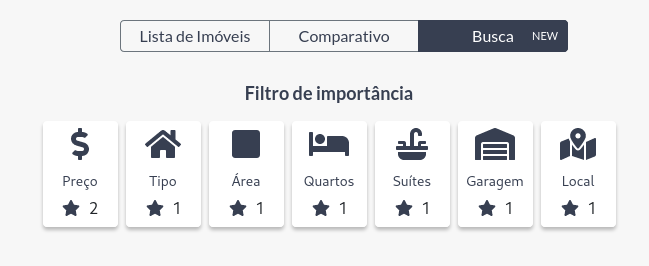
\includegraphics[scale=0.5]{figuras/desenvolvimento/componente_filtro.png}
    \caption[Nova aba de busca e o filtro de importância]{Nova aba de busca e o filtro de importância.}
    \label{fig:componente_filtro}
\end{figure}

\begin{figure}[H]
    \centering
    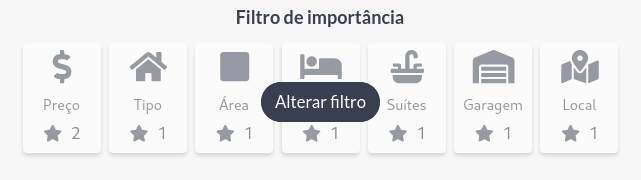
\includegraphics[scale=0.5]{figuras/desenvolvimento/componente_filtro2.png}
    \caption[Filtro de importância ao passar mouse]{Filtro de importância ao passar mouse.}
    \label{fig:componente_filtro2}
\end{figure}

\begin{figure}[H]
    \centering
    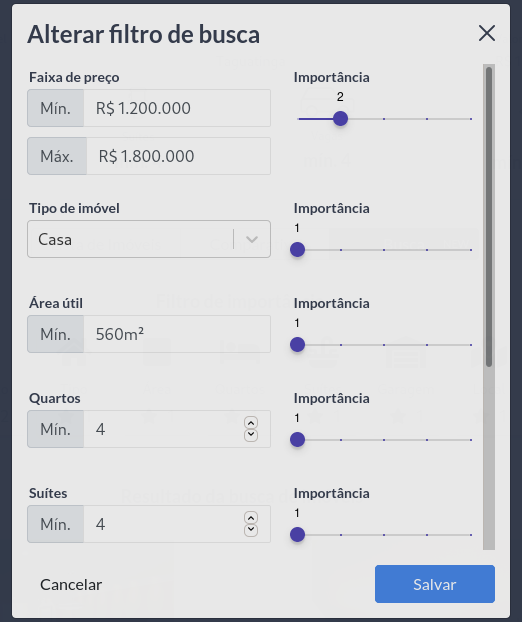
\includegraphics[scale=0.35]{figuras/desenvolvimento/componente_filtro3.png}
    \caption[Modal de alteração de filtro de busca - parte 1]{Modal de alteração de filtro de busca - parte 1.}
    \label{fig:componente_filtro3}
\end{figure}

\begin{figure}[H]
    \centering
    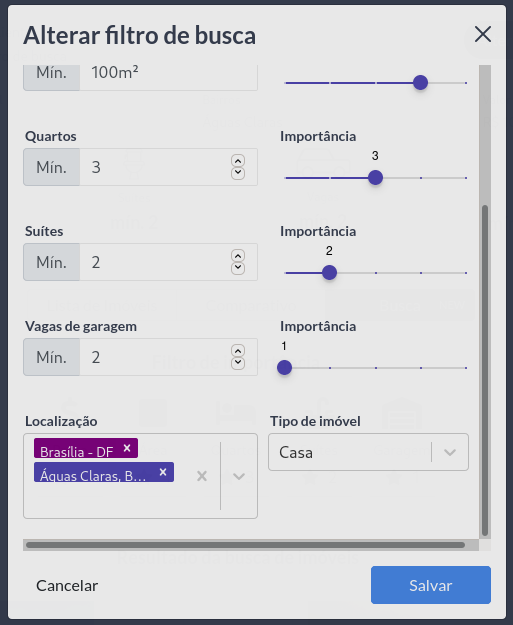
\includegraphics[scale=0.35]{figuras/desenvolvimento/componente_filtro4.png}
    \caption[Modal de alteração de filtro de busca - parte 2]{Modal de alteração de filtro de busca - parte 2.}
    \label{fig:componente_filtro4}
\end{figure}

\begin{figure}[H]
    \centering
    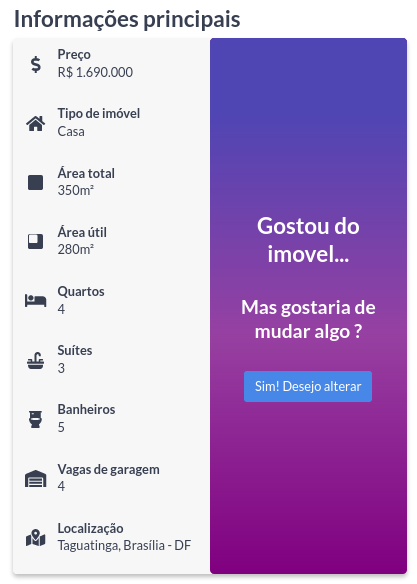
\includegraphics[scale=0.45]{figuras/desenvolvimento/componente_critica.png}
    \caption[Componente de descrição e crítica - parte 1]{Componente de descrição e crítica - parte 1.}
    \label{fig:componente_critica}
\end{figure}

\begin{figure}[H]
    \centering
    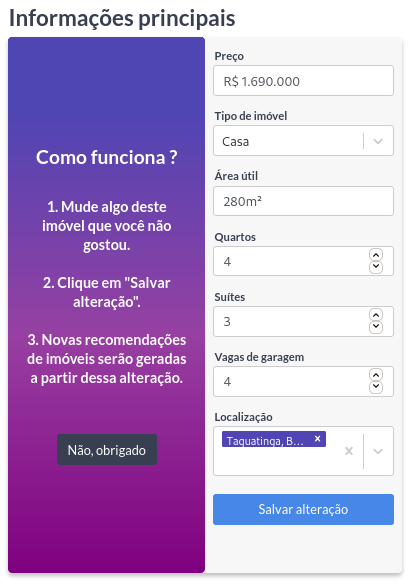
\includegraphics[scale=0.45]{figuras/desenvolvimento/componente_critica2.png}
    \caption[Componente de descrição e crítica - parte 2]{Componente de descrição e crítica - parte 2.}
    \label{fig:componente_critica2}
\end{figure}

Essa ferramenta de busca se baseia nas características do perfil de busca, igualmente como acontece no algoritmo de recomendação do \textit{feed}, mas difere-se no quesito em que o algoritmo utilizado é conforme o proposto nesse trabalho (\ref{exemple-critiquing}), ou seja, aplicando as técnicas de recomendações descritas. Um dos motivadores da utilização de uma ferramente de busca é pelo fator de que, como descrito no tópico \ref{Hybrid}, o sistema de recomendação baseado em crítica tem uma melhor performance quando utilizado juntamente com uma ferramenta de busca. Essa técnica foi feita para funcionar com tal tipo de ferramenta.

Em seguida, foi feita a implementação de todas as funções de pontuação referentes aos parâmetros do perfil de busca. Para dados quantitativos como quantidade de quartos, suítes e vagas na garagem, foi utilizado uma pontuação tendendo ao valor escolhido, ou seja, há uma pontuação máxima (100) caso o candidato tenha o valor escolhido no perfil de busca, e caso ele tenha diferença positiva, diminui da pontuação gradativamente.

Primeiramente, para calcular a pontuação referente a localização, foi utilizada uma equação linear, onde o valor resultante está entre 0 a 100. A localização da propriedade do candidato com menor distância ganha a maior pontuação (100) e a maior distância ganha a menor pontuação (0) sendo baseado nisso os outros candidatos ganham sua pontuação. Após testes manuais e reuniões foi notado que esse sistema de pontuação para localidade de imoveis não é adequado, pois existem bairros com diferenças econômicas muito grandes, ou seja, se tem um bairro colado a um outro, o sistema descrito anteriormente pode recomendar imoveis de um bairro para o outro e eles podem ser muito diferentes. Por esse motivo, foi decidido que esse filtro será estático, em que os candidatos a recomendação estarão somente na localização definida pelo usuário. O tipo do imóvel foi outro filtro escolhido como estático, pois assim como a localização e por se tratar de uma ferramenta de busca, em que o usuário vai experimentando a ferramenta e descobrindo seu alcance, se encaixam mais como estáticos, filtrando somente o tipo que foi selecionado.

Para o preço, assim como anteriormente para a localização, foi feita uma equação linear utilizando-se dos parâmetros mínimo e máximo do perfil de busca, em que o preço de venda do imóvel candidato mais perto do preço mínimo definido no perfil de busca tende ao máximo de pontuação (100). Valores fora do mínimo e máximo são considerados de pontuação 0.

Para calcular a pontuação da área, por se tratar de um valor quadrático, foi retirado o grau da área do candidato pela areá miníma definida no perfil de busca. Caso o resultado passe de 100, por se tratar de uma área miníma, mantém o valor de 100 para a pontuação.

Para realizar o \textit{deploy} no AWS, primeiro foi criado um repositório no ECR com o objetivo de armazenar e versionar a imagem do Docker do projeto. Ao mesmo tempo foi criado uma instância (servidor virtual na nuvem) no RDS para comportar o banco de dados Postgres. Com o registro da imagem armazenada, foi possível subir a API através do serviço ECS que ira mantê-lo em uma nova instância descrita em \ref{desempenho}.

\subsection{\textit{Sprint backlog} e resultados}

Passada a terceira \textit{sprint} em que foi possível fazer testes manuais no recomendador de aprendizado de maquina, foi possível observar e calcular o tempo de resposta do algoritmo de predição que não estava adequado. Com isso, para essa \textit{sprint} surgiu a \textit{story} técnica TS10 com o objetivo de aumentar o desempenho da predição. Também é priorizado a US04 e US06 do recomendador de critica com o foco de finalizar o sistema para colocá-lo para coletar dados em produção. No decorrer da \textit{sprint} com uma reunião antes de colocar o sistema em produção, um novo requisito surge para não ferir a regra de negocio da Liva, que é referente a nova ferramenta de busca com as \textit{stories} de usuário US07 e US08.  O quadro \ref{quadro:sprint4} apresenta o \textit{backlog} e resultados da quarta  \textit{sprint}.

\begin{quadro}[H]
\centering
\caption[\textit{Sprint backlog} e resultados da \textit{sprint} 4]{\textit{Sprint backlog} e resultados da \textit{sprint} 4.}
\label{quadro:sprint4}
\begin{tabular}{|p{6cm}|p{2cm}|p{2cm}|p{1cm}|}
\hline
\multicolumn{1}{|c|}{\textbf{Stories planejadas}} & \multicolumn{1}{c|}{\textbf{Concluídas}} & \multicolumn{1}{c|}{\textbf{Pendentes}} & \multicolumn{1}{c|}{\textbf{Novas}} \\ \hline
TS10 - Aumentar desempenho na parte de predição & X &  & X \\ \hline
US04 - Criticar características da propriedade & X &  & \\ \hline
US06 - Visualizar filtro de importância & X &  & X \\ \hline
US07 - Alterar filtro de importância & X &  & X \\ \hline
US08 - Acessar aba de busca no feed & X &  & X \\ \hline
\end{tabular}
\end{quadro}


\section{5º \textit{Sprint}}

Com o novo sistema de recomendação posto em produção no site da Liva foram possíveis fazer diversas análises iniciais. Uma delas foi relacionada ao fluxo de pessoas utilizando as recomendações, que estava baixo. Dessa forma, veio a decisão de adicionar um componente na lateral da página de detalhes e abaixo do componente de agendar visitas e tirar dúvidas, com o intuito de chamar a atenção do usuário, na qual um botão que se clicado rolará a página de detalhes para a posição do componente de apresentação de imóveis como na Figura \ref{fig:componente_scroll}.

\begin{figure}[H]
    \centering
    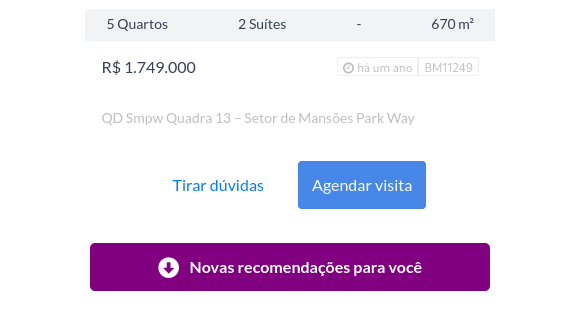
\includegraphics[scale=0.6]{figuras/desenvolvimento/componente_scroll.png}
    \caption[Componente de encaminhamento]{Componente de encaminhamento.}
    \label{fig:componente_scroll}
\end{figure}

Outra análise foi relacionada ao modelo de aprendizado de máquina, em que após alguns testes em um período longo de uso foi notado que quando o usuário chega a uma quantidade alta de cliques em propriedades, tende muito a recomendação das mesmas propriedades, ou seja, estava ocorrendo um \textit{overfitting}. Dessa maneira, a solução foi descartar alguns dados que não correspondiam com o "normal" e tinham muito mais interações  que o comum e ainda diminuir para 30 o número de interações de cliques do modelo.

Por último, foi determinado melhorar o sistema adotado de localização, que como descrito anteriormente, para o perfil de busca que comporta vários bairros ou cidade é tirada a média de sua latitude e longitude. Para melhorar ainda mais a precisão do modelo foi decidido que um usuário clicar em uma propriedade, e a localidade dessa propriedade se encontra em seu perfil de busca, então ela é escolhida para entrada do modelo, assim deixando a localidade mais precisa e condizente com a realidade.

\subsection{\textit{Sprint backlog} e resultados}

Com o sistema completo em produção, algumas modificações surgiram como necessárias. Primeiramente com a observação relacionada ao baixo fluxo de uso do componente de recomendação surge a US09 para implementação o botão para rolar a página. Outra \textit{story} técnica surge (TS11) com a observação da tendencia do recomendador de aprendizado de máquina quando há muitos cliques pelo cliente, demonstrando um  \textit{overfitting}. O quadro \ref{quadro:sprint5} apresenta o \textit{backlog} e resultados da quinta  \textit{sprint}.

\begin{quadro}[H]
\centering
\caption[\textit{Sprint backlog} e resultados da \textit{sprint} 5]{\textit{Sprint backlog} e resultados da \textit{sprint} 5.}
\label{quadro:sprint5}
\begin{tabular}{|p{6cm}|p{2cm}|p{2cm}|p{1cm}|}
\hline
\multicolumn{1}{|c|}{\textbf{Stories planejadas}} & \multicolumn{1}{c|}{\textbf{Concluídas}} & \multicolumn{1}{c|}{\textbf{Pendentes}} & \multicolumn{1}{c|}{\textbf{Novas}} \\ \hline
US09 - Rolar página do imóvel para visualizar recomendações & X &  & X \\ \hline
TS11 - Limpeza do \textit{dataset} & X &  & X \\ \hline
\end{tabular}
\end{quadro}

\section{Análises gerais}
\label{analise_gerais}

O novo sistema de recomendação foi colocado em produção por completo, com os dois sistemas de recomendação funcionando, na data de 08/10/2020 e foram coletados dados para serem analisados até a data de 11/11/2020. Neste período foram feitas diversas alterações nos recomendadores, como descrito anteriormente, sempre com o intuito de melhorá-los. Foram feitas mudanças na base de dados inicial, no algoritmo de predição, no design de componentes, nas funções de pontuação e dentre outras alterações importantes.

Para ser possível a medição das métricas descritas anteriormente em (\ref{metodologia}), além de novas análises, foram coletados dados do período de 03/09/2020 até 08/10/2020, para compara-los com os do período em que o novo sistema de recomendação entrou em produção. Para a coleta desses dados foi utilizada a ferramenta MixPanel, na qual foi utilizada também na simulação (Apêndice \ref{apendiceA}), além de buscas no banco de dados da Liva.

Logo de início, ao buscar dados relacionados a quantidade de conversões positivas e não conversões e suas origens, dos diferentes períodos, temos a seguintes gráficos referentes as Figuras \ref{fig:grafico1} e \ref{fig:grafico2}:

\begin{figure}[H]
    \centering
    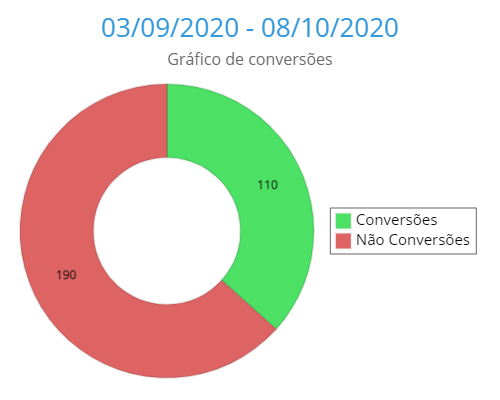
\includegraphics[scale=0.6]{figuras/desenvolvimento/grafico1.png}
    \caption[Gráfico de conversões antes do novo recomendador]{Gráfico de conversões antes do novo recomendador.}
    \label{fig:grafico1}
\end{figure}

\begin{figure}[H]
    \centering
    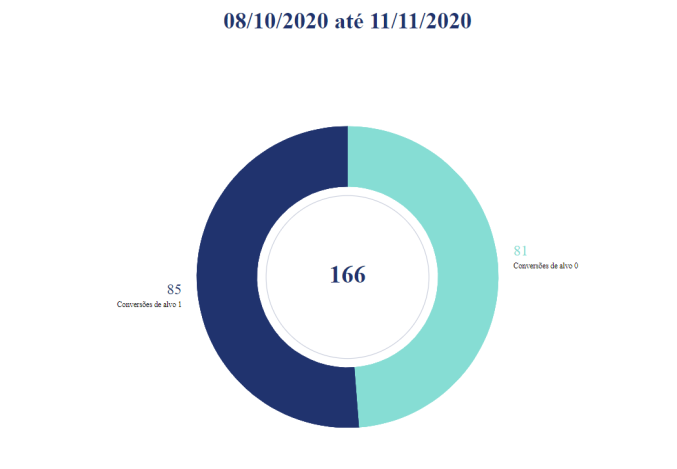
\includegraphics[scale=0.6]{figuras/desenvolvimento/grafico2.png}
    \caption[Gráfico de conversões durante o novo recomendador]{Gráfico de conversões durante o novo recomendado.}
    \label{fig:grafico2}
\end{figure}

Comparando as quantidades dentre conversões positivas e não conversões dos diferentes períodos é possível notar, primeiramente, para o período anterior a nova recomendação, uma quantidade muito maior de descartes de imoveis, o que mudou muito para o segundo período, em que as conversões se mantém equilibradas, ou seja, houve uma menor taxa de descartes, pro segundo período, como ocorrido também na simulação descrita no Apêndice (\ref{apendiceA}).

Para calcular a métrica de CVR ou \textit{conversion rate} descrita na seção \ref{metodologia}, coletamos, além das conversões, todos os cliques em recomendações dos usuários, demonstrados na Tabela (\ref{tab:my-table3}).

\begin{table}[H]
\centering
\caption[\textit{conversion rate}]{Conversion Rate.}
\begin{tabular}{lcc}
\hline
\textbf{Data do início - Data do fim} & 03/09/2020 - 08/10/2020 & 08/10/2020 - 11/11/2020 \\ \hline
\textbf{Quantidade de cliques} & 623 & 293 \\ \hline
\textbf{Quantidade de Conversões} & 110 & 85 \\ \hline
\textbf{CVR Aproximado} & 18\% & 29\% \\ \hline
\end{tabular}
\label{tab:my-table3}
\end{table}

Comparando os resultados do CVR é possível notar uma melhora de 11\% com a Liva compondo o novo sistema de recomendação elaborado. Na Tabela \ref{tab:my-table3} é possível também perceber uma grande diminuição na quantidade de cliques, isso pode ser interpretado pelo motivo dos usuários estarem demorando menos tempo para encontrar o imóvel a ser convertido. Dessa forma, foi decidido trazer os dados referentes a frequência de usuários diários nos dois períodos.

\begin{figure}[H]
    \centering
    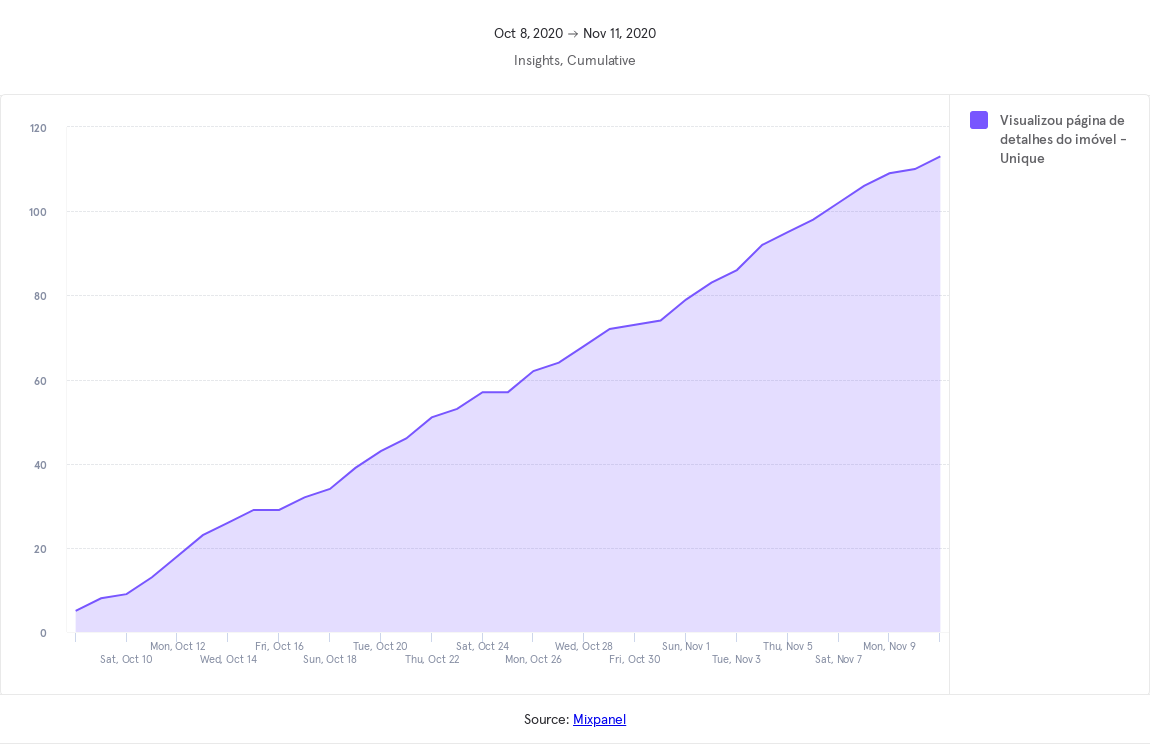
\includegraphics[scale=0.38]{figuras/desenvolvimento/mixpanel-antes.png}
    \caption[Gráfico de frequência dos usuários durante do novo recomendador]{Gráfico de frequência dos usuários durante do novo recomendador.}
    \label{fig:mixpanel-antes}
\end{figure}

\begin{figure}[H]
    \centering
    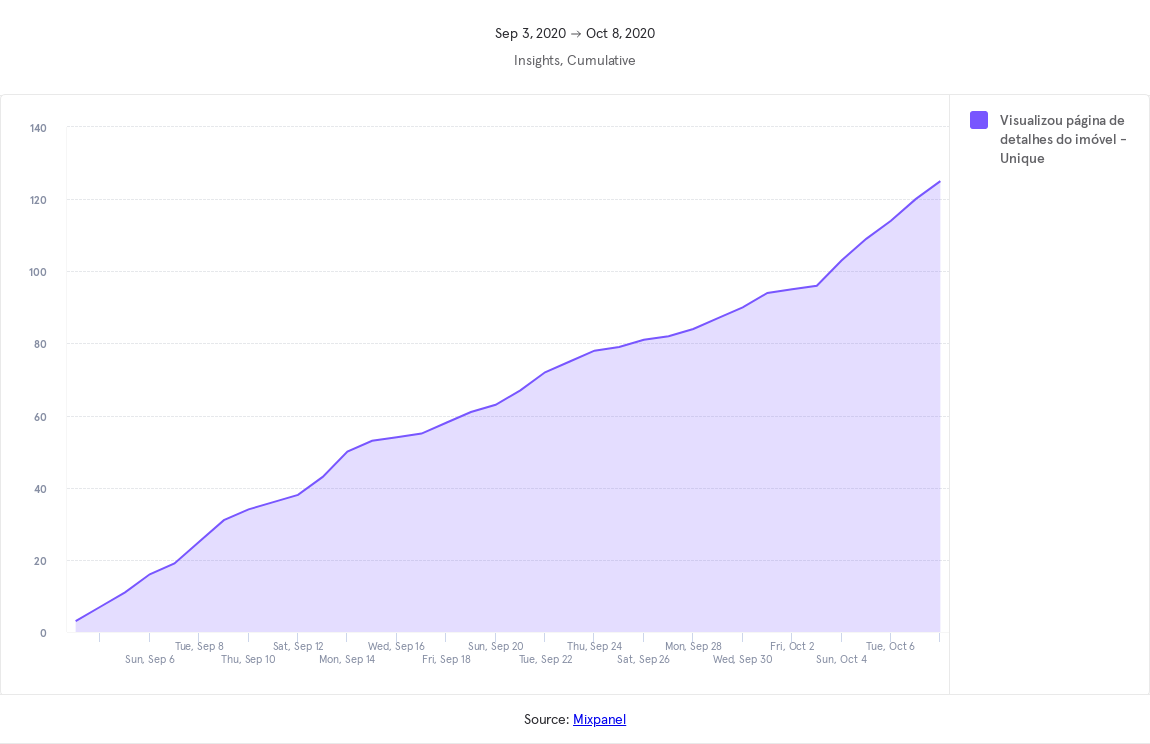
\includegraphics[scale=0.38]{figuras/desenvolvimento/mixpanel-depois.png}
    \caption[Gráfico de frequência dos usuários antes do novo recomendador]{Gráfico de frequência dos usuários antes do novo recomendador.}
    \label{fig:mixpanel-depois}
\end{figure}

Para o período anterior a nova recomendação existem 125 usuários ativos e para o período durante o uso, 113, como demonstrados nas Figuras \ref{fig:mixpanel-antes} e \ref{fig:mixpanel-depois}. Esses dados reforçam ainda mais que a grande diminuição na quantidade de cliques nos dois períodos é relacionada ao tempo do usuário encontrar o imóvel ideal, pois o fluxo de usuários se manteve muito parecido, com apenas 12 usuários de diferença.

% usuarios ativos
% 125 - 113

% cvs1 = 85
% feed = 68, 114
% help = 9
% visit = 8

% cvs0 = 81

% views  = 176

% cv sem click = 117

% CVR = 29%

% Clicks on recomendation ml = 22

% search profiles = 154
% que veio do feed = 48
% que veio do critica = 7 <= da data 

% OLDDDD
% feed = 98
% visit = 12

% CVR = 18\%

% views = 623

% cvs0= 190

% Para alcançar os objetivos descritos na seção \ref{section:objetivos}, que referem-se ao desenvolvimento de um sistema de recomendação, foi realizada inicialmente toda pesquisa bibliográfica necessária, além da realização da documentação referente a arquitetura do projeto, e dessa forma a descrição de como seria todo funcionamento do sistema e seu processo de análise, projeto e desenvolvimento com uma metodologia adequada.

% O objetivo principal desse trabalho é a construção de um sistema de recomendação robusto que funcionará como um serviço mais interessante para o ambiente virtual da Liva.vc, em que possa proporcionar para o usuário uma melhor experiência de uso com recomendações mais coerente com as demandas e preferências de seus usuários.

% Com a realização de implantação de um protótipo implementado para fins de simulação em ambiente da Liva, foi possível, com a análise dos dados coletados durante o experimento, a confirmação da viabilidade parcial de realização do projeto. Como o período do experimento foi pequeno, não foi possível apresentar um espaço amostral maior em que o processo de escolha de um imóvel para compra por um usuário é longo e necessita de muitas interações, o que normalmente leva um tempo maior.

% Para a segunda parte da monografia espera-se, com o desenvolvimento e aplicação do sistema de recomendação em ambiente de produção sítio virtual da Liva, a apresentação de um melhor resultado obtido pela mesma métrica adotada por Li et al. (\citeyear{Summo:2017}). Com ela será possível mensurar melhor a eficiência de um recomendador comparado ao outro previamente atribuído.

% Dessa forma, ao se apresentar melhores resultados iniciais é possível manter a motivação e a expectativa de que o desenvolvimento e implantação do novo sistema de recomendação no modelo híbrido proposto obterá melhores resultados para os usuários do ambiente virtual da Liva.
